\section{Project Requirements} \label{project-requirements}
\subsection{Software Requirements}
In order to run the code and reproduce results, software requirements must be installed and hardware requirements must be met as prerequisites to the project. While some software, like the development environments, are optional and are not needed to train the models, some modification to the code might be needed to run without them.

\phantomsection
\subsubsection{Python}
The entirety of the project's code was written in Python and such is a hard requirement to run the project's code. It is recommended to use Python 3.7 or later for TensorFlow support.

\subsubsection{TensorFlow and Keras}
The TensorFlow and Keras were used for the entirety of this project and such is a hard requirement to run the code. TensorFlow 2.0 and Keras 2.0 or later are recommended, with some code modifications; but TensorFlow 1.0+ and Keras 1.0+ can also be used.

\subsubsection{TensorBoard}
In this project, TensorBoard 2.8.0 was used and is a hard requirement to run the artefact. As with TensorFlow, it is recommended TensorBoard 2.0 or later is used, however with some code modifications, TensorBoard 1.0+ can also be used

\subsubsection{Scikit-Learn}
In this project, Scikit-Learn 1.0.2 was used and is a hard requirement to run the artefact.

\subsubsection{pandas}
In this project, pandas 1.3.5 was used and is a hard requirement to run the artefact.

\subsubsection{NumPy}
In this project, NumPy 1.21.6 was used and is a hard requirement to run the artefact.

\subsubsection{Google Cloud Platform - Development Environment}
Google Cloud Platform and its subsidiary solutions are not a requirement to run the artefact, however can be used to run model training simultaneously.

\subsubsection{Google Colab - Development Environment}
Google Colab is not a requirement to run the artefact, however a Jupyter notebook solution, such as Google Colab, must be used.

\subsubsection{Project Code}
The project code is hosted on GitHub, and can be accessed and downloaded through the following link: \url{https://github.com/laurencebrwn/ml-covid19-eval}. The results and individual models notebook files are all found here.

\subsubsection{COVIDx-CXR Dataset}
The dataset used to train the image classification models is a hard requirement for this project. The full dataset is hosted on kaggle, and can be found here: \url{https://github.com/lindawangg/COVID-Net/blob/master/docs/COVIDx.md}. The images should be obtained from the "COVIDx CXR-2 Kaggle Dataset" link (\url{https://www.kaggle.com/datasets/andyczhao/covidx-cxr2}) detailed on the previously linked page. The labels for both binary ("train\_COVIDx9B.txt" and "test\_COVIDx9B.txt") and multi-label ("train\_COVIDx9A.txt" and "test\_COVIDx9A.txt") classification, can be downloaded from the link (\url{https://github.com/lindawangg/COVID-Net/tree/master/labels}) detailed on the previously linked page.

\subsection{Hardware Requirements}
While TensorFlow can run on a large number of devices, there are some hardware limitations, especially if a Graphical Processing Unit (GPU) is used to accelerate performance. TensorFlow requires a CPU capable of AVX instructions, which most modern Computational Processing Units (CPU) support \citep{InstallT17:online}. If GPU acceleration is required and the device used has an NVIDIA GPU, then it must support compute unified device architecture (CUDA), a "parallel computing platform" which can "dramatically speed up computing applications by harnessing the power of GPUs" \citep{CUDAZone2:online}. If the device has a GPU that does not support CUDA, but does support DirectX 12 (e.g. an AMD GPU manufactured in the last several years), then Microsoft's DirectML can be used to enable GPU support for TensorFlow \citep{Introduc93:online}. However, precautions must be taken if DirectML is used as it has differing version requirements of Python, TensorFlow and NumPy.

\section{Design} \label{design}
To design software capable of training and evaluating each of the selected models, as identified in the literature review, prompts were taken from the methodology to devise a structure to form each model’s notebook. By implementing a general structure that all models would inherit, it made changes to the models and hyper parameters easy, while reducing development time. Although there are a few variations for each model, a common format was followed for all models:

\begin{enumerate}
    \item Set up the environment.
    \begin{enumerate}
        \item Define the model and training variables.
        \item Import the required libraries, like TensorFlow, Keras, Scikit-Learn, etc.
        \item Define the hyper-parameters of the model (or list of hyper-parameters if performing tuning).
    \end{enumerate}
    \item Prepare the dataset.
    \begin{enumerate}
        \item Read in the label files for both test and train.
        \item Down-sample each class to match the total dataset size and to ensure all classes are equally represented.
        \item Shuffle the data.
        \item Pre-process the X-Ray images (and perform image transformations on the training dataset).
        \item Split the training data into folds for stratified K fold cross validation.
    \end{enumerate}
    \item Create the machine learning model.
    \begin{enumerate}
        \item Create the Keras sequential model.
        \item If the model is using transfer learning (Xception, ResNet and DenseNet), fetch the base model from Keras' application library.
        \item Define the model layers in the sequential model.
        \item Set any hyper-parameters, like the optimiser, learning rate etc.
        \item Compile the model.
    \end{enumerate}
    \item Begin cross validation training.
    \begin{enumerate}
        \item Iterate through hyper-parameter variations.
        \item Iterate through stratified K folds.
        \item Train the model.
        \item Record model logs.
        \item Save the model weights.
    \end{enumerate}
    \item Evaluate the model.
    \begin{enumerate}
        \item Iterate through the trained models.
        \item Load model weights.
        \item Predict the labels on the test dataset.
        \item Record the model's key metrics, described in the methodology.
        \item Save the model's metrics and performance
    \end{enumerate}
\end{enumerate}

\section{Developing the Artefact}
Developing the Python notebooks for each model followed a similar flow to that listed in the \autoref{design} Design. Firstly the environment set up was developed, followed by dataset preparation and pre-processing. However, the development flow differed, as the cross validation training and evaluation sections were developed before the model itself. This meant a skeletal structure consisting of everything except for the model itself could be replicated, once for each model. The development of the artefact is detailed below, through a run through of the code itself, split into the sections listed in the design format (as specified in \autoref{design}).

\subsection{Environment Set Up}
Firstly the correct environment had to be set up before any machine learning models were created or training was to happen. This started with defining the image size, batch size, dataset size, number of K folds, the maximum number of epochs and the path to the dataset. Secondly the required libraries were imported. This included NumPy, pandas, TensorFlow, Scikit-Learn, TensorBoard and other generic Python libraries, such as those used to record the time. Finally the hyper-parameters were instantiated. This was done using TensorBoard's "hparams" plugin. An example of this can be seen in \autoref{fig:hyper-param-code}.

\begin{figure}[H]
    \centering
    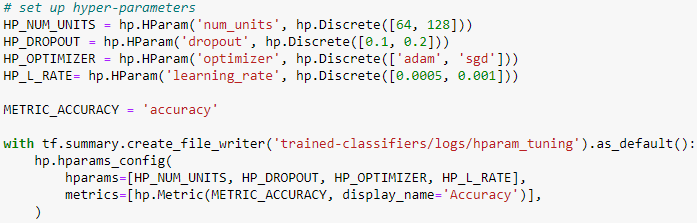
\includegraphics[width=\textwidth]{figures/hyper-param-code.png}
    \caption{Defining the hyper-parameters with TensorBoard.}
    \label{fig:hyper-param-code}
\end{figure}

\subsection{Dataset Preparation}
Next the COVIDx-CXR dataset had to be brought in and manipulated so the models could use it for training. To begin, the dataset labels were read in and unnecessary columns, like "patient id" and "data source", were removed. Next the data was down-sampled, so the classes were of equal proportions, and thoroughly shuffled. This was done with Scikit-Learns "resample" function, an example of this can be seen in \autoref{fig:dataset-downsampling}. 

\begin{figure}[H]
    \centering
    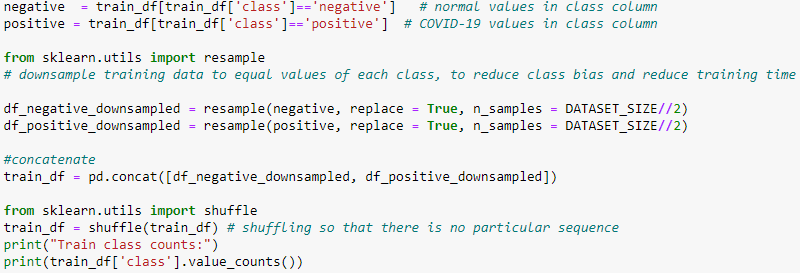
\includegraphics[width=\textwidth]{figures/dataset-downsampling.png}
    \caption{Down-sampling and shuffling the dataset.}
    \label{fig:dataset-downsampling}
\end{figure}

The dataset labels then had to be linked with the corresponding images. This was done with Keras' "ImageDataGenerator". Using "ImageDataGenerator" allowed for the use of the "flow\_from\_dataframe()" function, which matches up the image paths, stored in a DataFrame, to the images themselves. It also allowed for image pre-processing to be performed serially, each time an image was flowed from the DataFrame. While the image pre-processing remained mostly constant for each model, some models, like Xception, ResNet50V2 and DenseNet201, each had a specific pre-processing, created for that model by Keras. Pre-processing the training images also took a different form from the test images, as the data had to be split into training and validation folds, dictated by the stratified K fold implementation. A separate function was made for this purpose, an example of which, used for the Xception model, can be seen in \autoref{fig:image-preprocessing}.

\begin{figure}[H]
    \centering
    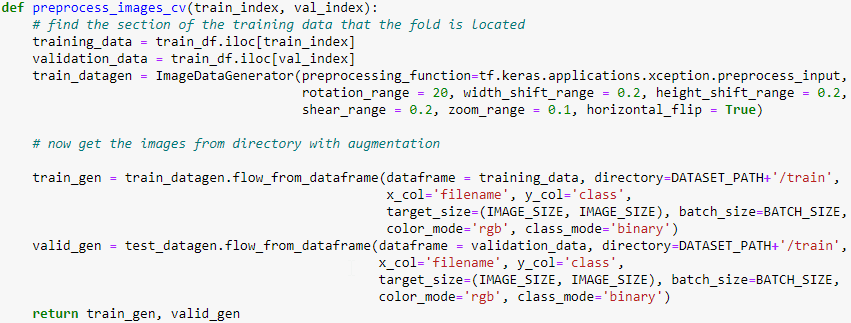
\includegraphics[width=\textwidth]{figures/image-preprocessing.png}
    \caption{Down-sampling and shuffling the dataset.}
    \label{fig:image-preprocessing}
\end{figure}

\subsection{Creating the Models}
Next each of the six models had to be built. While each models architecture differed, each model used some or all of the same layers. To understand this better research was carried out on each layer's functions. The following is an explanation for layers used in the models:

\begin{itemize}
    \item Dense -  A deeply connected neural network layer (all neurons receive inputs from all neurons in the previous layer) that performs matrix-vector multiplication, with the values of said matrix being trained and updated with back propagation \citep{Denselay11:online}.
    \item Conv2D - Creates a convolution kernel that is convolved with the input, in this case an image, or the previous layer's output. The result of the kernel produces a tensor of outputs \citep{Conv2Dla69:online}.
    \item GlobalAveragePooling2D - Down-samples the entire feature map to a single value. In a 2D layer it takes a 4D tensor and returns a 2D tensor with the shape of (batch size, number of channels) \citep{GlobalAv91:online}.
    \item BatchNormalization - Normalises its inputs by applying a transformation that maintains the outputs mean to as close to 0 as possible and its standard deviation as close to 1 as possible \citep{BatchNor52:online}.
    \item Dropout - Randomly sets input values to 0, at a user defined frequency, to prevent over-fitting. Those inputs that are not set to 0 are scaled so the total sum of the inputs is unchanged \citep{Dropoutl66:online}.
    \item Activation - Applies a user defined activation function to the input, while retaining the input shape \citep{Activati33:online}.
    \item MaxPooling2D - Similar to GlobalAveragePooling 2D, in that it down-samples the entire feature map, but this time takes the maximum value over a user defined input window, known as a pool size \citep{MaxPooli1:online}.
    \item Flatten - Flattens the input to a 1D shape, while retaining the batch size \citep{Flattenl52:online}.
\end{itemize}

The models were created inside a create\_model() function which takes the hyper-parameters as an input, and returns the model as an output. Inside the function the Keras sequential or functional API is used to create the model, before defining its optimiser and learning rate, before compiling the model. An example of this, used for the Xception model can be seen in \autoref{fig:createmodel-function}.

\begin{figure}[H]
    \centering
    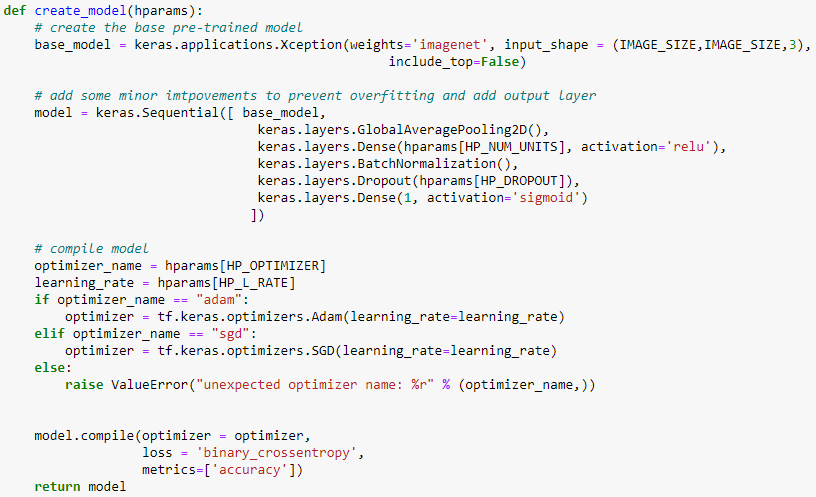
\includegraphics[width=\textwidth]{figures/xception-model.png}
    \caption{The create\_model() function structure, used for creating Xception in this case.}
    \label{fig:createmodel-function}
\end{figure}

While model architecture of the used models was standard, each model was slightly modified initially for better performance, and to match the correct output specification (ie. number of classes). Each model has a different architecture and layer structure, and the following sections will explain in detail the model architecture for each, including any modifications made.

\phantomsection
\subsubsection{AlexNet}
Since Keras has no application model available for AlexNet, it had to be reproduced manually using Keras' sequential API. A description of the architecture, taken from \cite{krizhevsky2012imagenet}, was used for this.

AlexNet consists of 5 Conv2D layers, each of which is followed by a BatchNormalization layer, an Activation layer with a rectified linear activation function (ReLU) and a MaxPooling2D layer, before being passed to the next Conv2D layer. Following this the output is flattened, and passed to 3 Dense layers, each of which is followed by a BatchNormalization layer, an Activation layer with a rectified linear activation function (ReLU) and a Dropout layer. This is finally followed by an output layer, which is a Dense layer with a single output (for binary classification), a BatchNormalization layer and an Activation layer with a sigmoid activation function.

Hyper-parameter tuning involved changing the final Dense layer's number of units, all three Dense layers dropout values, the optimiser and the learning rate. The full model code can be seen in \autoref{fig:alexnet-model-part1} and \autoref{fig:alexnet-model-part2}.

\subsubsection{DenseNet201}
DenseNet201 is included in Keras' application models, so could be imported with pre-trained weights, without having to be reproduced. The architecture Keras uses is taken from \cite{huang2017densely}.

To build the implementation for DenseNet201 used in this project, the base model was imported from Keras' applications, with the pre-trained weights from training on the ImageNet dataset. It was then added to a Keras sequential API where some additional layers were added, to prevent over-fitting and produce a usable output. This was achieved by adding a GlobalAveragePooling2D layer that received DenseNet201's output, followed by a Dense layer with a rectified linear activation function (ReLU), followed by a BatchNormalization layer and a Dropout layer. This was finally followed by an output layer, which is a Dense layer with a single output (for binary classification) and a sigmoid activation function.

Hyper-parameter tuning involved changing the final Dense layer's number of units, the Dropout layers dropout values, the optimiser and the learning rate. The full model code can be seen in \autoref{fig:densenet-model}.

\subsubsection{ResNet50V2}
The implementation of ResNet50V2 follows a similar route to DenseNet201, as the model is available from Keras' application models. The architecture Keras uses is taken from \cite{he2016identity}.

To build the implementation for ResNet50V2 used in this project, the base model was imported from Keras' applications, with the pre-trained weights from training on the ImageNet dataset. It was then added to a Keras sequential API, where additional layers were added to prevent over-fitting and produce a usable output. This was achieved by adding a GlobalAveragePooling2D layer that received ResNet50V2's output, followed by a Dense layer with a rectified linear activation function (ReLU), followed by a BatchNormalization layer and a Dropout layer. This was finally followed by an output layer, which is a Dense layer with a single output (for binary classification) and a sigmoid activation function.

Hyper-parameter tuning involved changing the final Dense layer's number of units, the Dropout layers dropout values, the optimiser and the learning rate. The full model code can be seen in \autoref{fig:resnet-model}.

\subsubsection{SqueezeNet}
Since Keras has no application model available for SqueezeNet, it had to be reproduced manually using Keras' functional API. A description of the architecture, taken from \cite{iandola2016squeezenet}, was used for this.

To build the implementation for SqueezeNet used in this project, the input shape was defined (image size and number of channels), followed by the SqueezeNet architecture. The SqueezeNet architecture consists of a Conv2D layer followed by five fire modules, separated by MaxPooling2D layers. A fire module is a key factor in SqueezeNet's small size. It consists of a squeeze layer, a Conv2D layer with a 1$\times$1 kernel size, squeezing the inputs. This was followed by an expand layer, which then expands the inputs back up, using a Conv2D layer with a 1$\times$1 kernel size and a Conv2D layer with a 3$\times$3 kernel size. The outputs of both Conv2D layers in the expand layer were then concatenated and results were returned. After the final fire modules, the output was down-sampled using a GlobalAveragePooling2D layer. Then the network was tweaked slightly by adding a Dropout layer, to reduce over-fitting, and a Dense layer with a single output (for binary classification) and a sigmoid activation function.

Hyper-parameter tuning involved changing the final Dropout layer's dropout values, the optimiser and the learning rate. The full model code can be seen in \autoref{fig:squeezenet-model}, and the fire module code in \autoref{fig:squeezenet-fire-module}.

\subsubsection{Xception}
The implementation of Xception follows a similar route to DenseNet201 and ResNet50V2, as the model is available from Keras' application models. The architecture Keras uses is taken from \cite{chollet2017xception}.

To build the implementation for Xception used in this project, the base model was imported from Keras' applications, with the pre-trained weights from training on the ImageNet dataset. It was then added to a Keras sequential API where additional layers were added, to prevent over-fitting and produce a usable output. This was achieved by adding a GlobalAveragePooling2D layer that received Xception's output, followed by a Dense layer with a rectified linear activation function (ReLU), followed by a BatchNormalization layer and a Dropout layer. This was finally followed by an output layer, which was a Dense layer with a single output (for binary classification) and a sigmoid activation function.

Hyper-parameter tuning involved changing the final Dense layer's number of units, the Dropout layer's dropout values, the optimiser and the learning rate. The full model code can be seen in \autoref{fig:xception-model}.

\subsubsection{ConvNet}
ConvNet is a basic CNN created for this project using Keras' sequential API, consisting of three convolutional layers.

To build ConvNet, a sequential model was instantiated, and three Conv2D layers were added. Following each Conv2D layer sat an Activation layer with a rectified linear activation function (ReLU) and a MaxPooling2D layer. The Conv2D layers had filter sizes of 32, 32 and 64 respectively, while all sharing the same 3$\times$3 kernel size. The output of the 3 Conv2D layers (in series) was then flattened and fed to the output portion of the model. The output portion of ConvNet was not too dissimilar from Xception, DenseNet201 and ResNet50V2. The output section aimed to reduce over-fitting and improve accuracy further, this was achieved by adding a Dense layer with a rectified linear activation function (ReLU) and a Dropout layer. This was finally followed by an output layer, which is a Dense layer with a single output (for binary classification) and a sigmoid activation function.

Hyper-parameter tuning involved changing the final Dense layers number of units, the Dropout layers dropout values, the optimiser and the learning rate. The full model code can be seen in \autoref{fig:convnet-model}.

\subsection{Cross Validation Training}
Next the model must be trained, and its hyper-parameters tuned, using stratified K fold cross validation. Firstly, to perform hyper-parameter tuning, all the hyper-parameter combinations must be iterated through. For each iteration of hyper-parameter combinations, cross validation was then performed. Using Scikit-Learns stratified K fold implementation, indexes for the training and validation dataset were created. These variations of indexes, put together to create 5 folds, were then iterated through. For each set of training and validation indexes, the images for each were collected using the pre-processing function discussed earlier. Logging for the model was set up, so that TensorBoard could record the fitting data of the models, over the epochs that the model trained. Details of the hyper-parameters used for each particular run were also stored. Several callbacks were used while training the model, the most notable were the following. Firstly, the model checkpoint callback, which saved the trained model weights of each model. Secondly, the early stopping callback, which finished the model training if the validation loss rate plateaued over three epochs. Third, the learning rate reduction callback, which reduced the learning rate by a factor of half if the validation loss plateaued over one epoch. The model was then trained, over a maximum of 20 epochs, using the previously discussed callbacks and training and validation datasets. Finally the location of where the model's weights were saved was recorded, so each trained model could be called upon during validation. A snippet of the cross validation code, where the folds are iterated through, the model trained and metrics recorded, can be seen in \autoref{fig:cv-function}.

\begin{figure}[H]
    \centering
    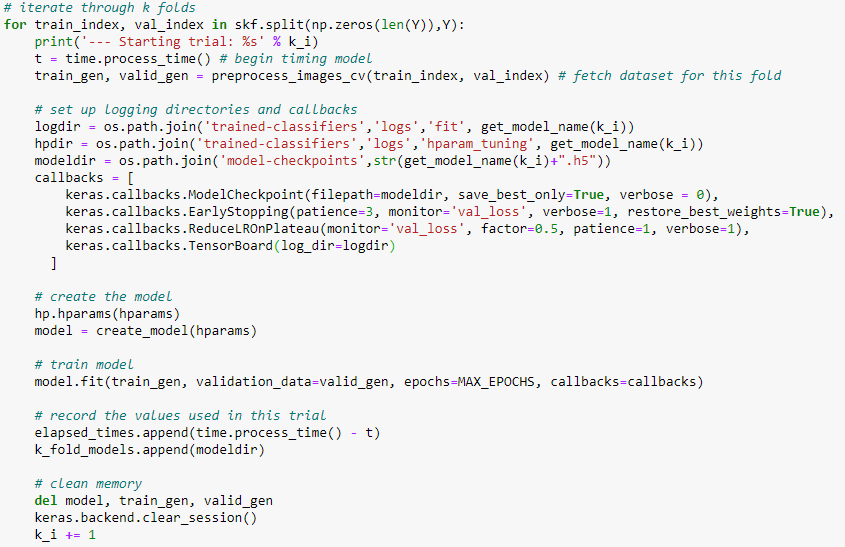
\includegraphics[width=\textwidth]{figures/cv-code.png}
    \caption{A snippet of the cross validation code.}
    \label{fig:cv-function}
\end{figure}

\subsection{Model Evaluation}
Finally the models were evaluated. This was done by iterating though all the hyper-parameter variations, and then calculating mean figures of accuracy, precision, recall F1 score and confusion matrices for all the folds of that variation. These metrics were then saved to a CSV file to be evaluated. A snippet showing the functions used for evaluation can be seen in \autoref{fig:metric-calculation}.

\begin{figure}[H]
    \centering
    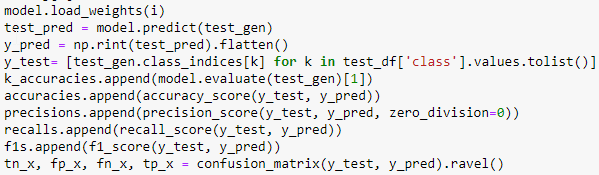
\includegraphics[width=0.8\textwidth]{figures/metric-calculation.png}
    \caption{A snippet showing the functions used for evaluation.}
    \label{fig:metric-calculation}
\end{figure}

\section{Testing}
The testing of the models followed the structure defined in section \ref{model-training}. After running each of the six models through hyper-parameter tuning on the small version of the datasets, it was found that the Xception model, with the following hyper-parameters was the best performing:

\begin{itemize}
    \item Number of Dense units - 128
    \item Dropout - 0.1
    \item Optimiser - Adam
    \item Learning rate - 0.001
\end{itemize}

While full results and analysis are discussed later (see \autoref{results}), this was the model selected for further improvement. The model went through five iterations of improvements before a final evaluation was performed. The five iterations of improvements were performed using a trial and error technique, using data identified during this phase as the basis for each improvement. The following sections detail each attempted improvement made to the Xception model.

\phantomsection
\subsubsection{Improvement 1 - Freezing Weights}
The first improvement to the Xception model was to freeze all the base model's trainable weights, seen in \autoref{fig:xception-freezing}, meaning that only weights in the added GlobalAveragePooling2D, Dense and Dropout layers could be trained. This recommendation was provided by Keras' own transfer learning guide, with the reasoning that it would prevent over-fitting to the training data \citep{Transfer59:online}. The full model code can be seen in \autoref{fig:xception-improvement-1}.

\begin{figure}[H]
    \centering
    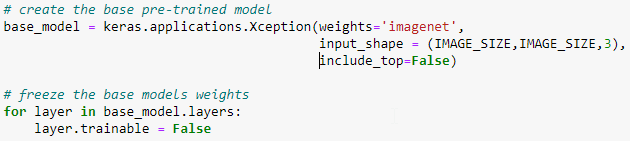
\includegraphics[width=\textwidth]{figures/xception-freezing.png}
    \caption{Freezing the base model's trainable weights.}
    \label{fig:xception-freezing}
\end{figure}

This yielded far worse results, possibly due to the fact that Xceptions pre-trained weights are from training on ImageNet, a dataset of images of objects, few of which, if any, could be X-Ray images. The changes were not carried onto the next round of improvements.

\subsubsection{Improvement 2 - Regularisation}
The second improvement made to the Xception model was to add regularisers to the Dense layer appended to the base model, seen in \autoref{fig:xception-regular}. Regularisers apply a penalty on the layer parameters and activity during model optimisation, this penalty is used in the loss function that the model works on optimising while training \citep{Layerwei14:online}. During this round another optimiser was also trialed as an extension to the hyper-parameter tuning, stochastic gradient descent with momentum. Using momentum in gradient descent algorithms can greatly improve training times by helping accelerate the gradient in the correct direction, instead of travelling at a fixed velocity \citep{qian1999momentum}. The full model code can be seen in \autoref{fig:xception-improvement-1}.

\begin{figure}[H]
    \centering
    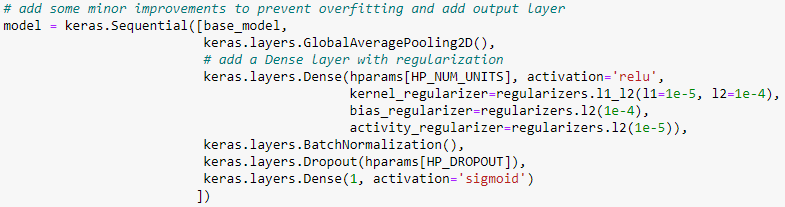
\includegraphics[width=\textwidth]{figures/xception-regular.png}
    \caption{Adding regularisers to the Dense layer.}
    \label{fig:xception-regular}
\end{figure}

The regularisation applied to the Dense layer resulted in slightly more varied results than without, possibly due to its effect on the model optimisation, with the base model's layers not being regularised. However, it demonstrated a marginal increase in speed. Using stochastic gradient descent with momentum did result in a faster training time over classic stochastic gradient descent, without affecting model performance. This however was still slower than the previous best optimiser selected in hyper-parameter tuning, the Adam optimiser, so was also not carried onto the next round of improvements

\subsubsection{Improvement 3 - Concatenated Models}
The third improvement drew inspiration from \cite[p. 343]{fitriasari2021improvement}, which proposes an architecture consisting of a "modified combination of two CNN architectures named Xception and ResNet50V2". This model was made using Keras' sequential API, where two separate "sub-models" consisting of a regularised version of Xception and ResNet50V2 used previously were concatenated. These were then passed through an additional 3 Dense layers and a Dropout layer before its final output. The full model code can be seen in \autoref{fig:xception-improvement-3-part1} and \autoref{fig:xception-improvement-3-part2}.

While training, the model learnt relatively slowly compared to other models; this was likely due it its large size. While model accuracy was not improved at all, further trial and error of this architecture lead to the next round of improvements.

\subsubsection{Improvement 4}
The fourth improvement was an exact replica of the \cite{fitriasari2021improvement} model. Here the two "sub-models" had no additional layers added before concatenation, and all trainable layers were frozen, with the exception of the last three. Following the "sub-models" concatenation, the output of the two were passed through a Conv2D layer, flattened and passed through a Dropout layer followed by 2 Dense layers, one with a ReLU activation function and the other with a sigmoid activation function. The first dense layer was regularised and the second was used as the output layer. The full model code can be seen in \autoref{fig:xception-improvement-4}.

Here the training time was halved, showing a significant improvement over all other models training time. This is likely due to the frozen training layers. While the model accuracy was only slightly less than improvement 3, the model showed an alarmingly high number of False Negatives, so was no longer considered for the final assessment.

\subsubsection{Improvement 5}
The final trial at improving the Xception model took cues from all the previous attempted improvements, by combining them into one model. Here none of the weights were frozen and the same layers were after the Xception model as in Improvement 4, which showed some speed increases with regularisation, and consistency with the Conv2D layer and Dense layers. The full model code can be seen in \autoref{fig:xception-improvement-5}.

The final round of improvements did show some promise, with significantly faster training times, but this came at a cost of a much worse mean accuracy in validation and testing. Eventually all improvements were abandoned, and the original alterations to the network where deemed the most suitable and performant.

\section{Operation of Artefact}
The operation of the model evaluation notebooks first depends on both the software and hardware requirements listed in section \ref{project-requirements}. Once hardware requirements are met, the Python notebooks downloaded can then be ran, to begin model training and evaluation. The models can be tuned using the model variables section, seen in \autoref{fig:model-variables}, and the hyper-parameters tuning section, seen in \autoref{fig:hyper-parameters-code}. One must pay close attention to the "DATASET\_PATH" variable and ensure it is pointed to the directory in which the COVIDx-CXR dataset resides.

\begin{figure}[H]
    \centering
    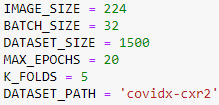
\includegraphics[width=0.3\textwidth]{figures/model-variables.png}
    \caption{Where to change model variables.}
    \label{fig:model-variables}
\end{figure}
\begin{figure}[H]
    \centering
    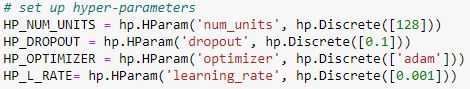
\includegraphics[width=0.6\textwidth]{figures/hyper-parameters-code.png}
    \caption{Where to change hyper-parameters.}
    \label{fig:hyper-parameters-code}
\end{figure}

\section{Results} \label{results}
The following are the results from the initial round of training, showing each of the six models, with only the best hyper-parameter variations. The full results of each model can be seen in \autoref{fig:xception-results}, \autoref{fig:densenet-results}, \autoref{fig:resnet-results}, \autoref{fig:squeezenet-results}, \autoref{fig:convnet-results} and \autoref{fig:alexnet-results} respectively. Note, here the Accuracy, Precision, Recall and F1 Scores are taken from a mean of the evaluation of each fold on the test dataset for conciseness.

\begin{longtable}[c]{l|l|l|l|l|l}
    \caption{Initial training results of the six models, with best hyper-parameters.} \\
    \begin{tabular}[c]{@{}l@{}}Model and\\ Hyper-Parameters\end{tabular} & Accuracy & Precision & Recall & \begin{tabular}[c]{@{}l@{}}F1\\ Score\end{tabular} & \begin{tabular}[c]{@{}l@{}}Training\\ Time (s)\end{tabular} \\ \hline\hline
    \endfirsthead
    %
    \multicolumn{6}{c}%
    {{\bfseries Table \thetable\ continued from previous page}} \\
    \begin{tabular}[c]{@{}l@{}}Model and\\ Hyper-Parameters\end{tabular} & Accuracy & Precision & Recall & \begin{tabular}[c]{@{}l@{}}F1\\ Score\end{tabular} & \begin{tabular}[c]{@{}l@{}}Training\\ Time (s)\end{tabular} \\ \hline\hline
    \endhead
    %
    \begin{tabular}[c]{@{}l@{}}Xception\\ \textit{Dense units - 128}\\ \textit{Dropout - 0.1}\\ \textit{Optimiser - Adam}\\  \textit{Learning rate - 0.001}\end{tabular} & 0.9780 & 0.9919 & 0.9640 & 0.9775 & 1202 \\
    \begin{tabular}[c]{@{}l@{}}DenseNet\\ \textit{Dense units - 128}\\ \textit{Dropout - 0.1}\\ \textit{Optimiser - Adam}\\ \textit{Learning rate - 0.0005}\end{tabular} & 0.9745 & 0.9900 & 0.9590 & 0.9738 & 762 \\
    \begin{tabular}[c]{@{}l@{}}ResNet\\ \textit{Dense units - 64}\\ \textit{Dropout - 0.2}\\ \textit{Optimiser - Adam}\\ \textit{Learning rate - 0.0005}\end{tabular} & 0.9510 & 0.9771 & 0.9240 & 0.9488 & 557 \\
    \begin{tabular}[c]{@{}l@{}}SqueezeNet\\ \textit{Dropout - 0.2}\\ \textit{Optimiser - Adam}\\ \textit{Learning rate - 0.0005}\end{tabular} & 0.9290 & 0.9036 & 0.9620 & 0.9316 & 282 \\
    \begin{tabular}[c]{@{}l@{}}ConvNet\\ \textit{Dense units - 128}\\ \textit{Dropout - 0.2}\\ \textit{Optimiser - RMS-Prop}\\ \textit{Learning rate - 0.0005}\end{tabular} & 0.7995 & 0.7823 & 0.8340 & 0.8060 & 331 \\
    \begin{tabular}[c]{@{}l@{}}AlexNet\\ \textit{Dense units - 1024}\\ \textit{Dropout - 0.2}\\ \textit{Optimiser - SGD}\\\textit{Learning rate - 0.001}\end{tabular} & 0.7095 & 0.8123 & 0.5480 & 0.6532 & 734
    \label{fig:initial-results-short}
\end{longtable}

The following are a summary of the results from the second round of training, showing each of the improvements performance on the Xception model. The full results of each improvement can be seen in \autoref{fig:xception-improvement-results}. Note, here the Accuracy, Precision, Recall and F1 Scores are taken from a mean of the evaluation of each fold on the test dataset for conciseness.

\begin{longtable}[c]{l|l|l|l|l|l}
    \caption{Improvement training results of the Xception model.} \\
    Model & Accuracy & Precision & Recall & \begin{tabular}[c]{@{}l@{}}F1\\ Score\end{tabular} & \begin{tabular}[c]{@{}l@{}}Training \\ Time (s)\end{tabular} \\ \hline\hline
    \endfirsthead
    %
    \multicolumn{6}{c}%
    {{\bfseries Table \thetable\ continued from previous page}} \\
    Model & Accuracy & Precision & Recall & \begin{tabular}[c]{@{}l@{}}F1\\ Score\end{tabular} & \begin{tabular}[c]{@{}l@{}}Training \\ Time (s)\end{tabular} \\ \hline\hline
    \endhead
    %
    \begin{tabular}[c]{@{}l@{}}Improvement 1\\ \textit{Adam}\end{tabular} & 0.5740 & 0.7293 & 0.2780 & 0.3600 & 177 \\
    \begin{tabular}[c]{@{}l@{}}Improvement 1\\ \textit{SGD \& Momentum}\end{tabular} & 0.5330 & 0.5903 & 0.1510 & 0.2241 & 187 \\
    \begin{tabular}[c]{@{}l@{}}Improvement 2\\ \textit{Adam}\end{tabular} & 0.9395 & 0.9837 & 0.8950 & 0.9331 & 1132 \\
    \begin{tabular}[c]{@{}l@{}}Improvement 2\\ \textit{SGD \& Momentum}\end{tabular} & 0.8670 & 0.9316 & 0.7920 & 0.8555 & 1200 \\
    Improvement 3 & 0.9095 & 0.9864 & 0.8310 & 0.8915 & 1389 \\
    Improvement 4 & 0.8240 & 0.7787 & 0.6660 & 0.7177 & 646 \\ 
    Improvement 5 & 0.6715 & 0.6826 & 0.5590 & 0.5161 & 922
    \label{fig:improvement-results-short}
\end{longtable}

The following are a summary of the results from the final round of training, showing the performance of the Xception model with the first, and best improvements (\autoref{fig:xception-model-final}), the performance of the Xception model with no improvements (\autoref{fig:xception-model-final-no-improv}) and the performance of the Xception model with no pre-trained weights (\autoref{fig:xception-model-final-no-weights}). Each of which are trained on both the small and large datasets of the binary classification label sets. The full results of each model can be seen in \autoref{fig:xception-model-final-results}. Note, here the Accuracy, Precision, Recall and F1 Scores are taken from a mean of the evaluation of each fold on the test dataset for conciseness.

\begin{longtable}[c]{l|l|l|l|l|l}
    \caption{Final training results of the binary classification performance of the Xception models, with improvements from this study, and without.} \\
    Model & Accuracy & Precision & Recall & \begin{tabular}[c]{@{}l@{}}F1\\ Score\end{tabular} & \begin{tabular}[c]{@{}l@{}}Training\\ Time (s)\end{tabular} \\ \hline\hline
    \endfirsthead
    %
    \multicolumn{6}{c}%
    {{\bfseries Table \thetable\ continued from previous page}} \\
    Model & Accuracy & Precision & Recall & \begin{tabular}[c]{@{}l@{}}F1\\ Score\end{tabular} & \begin{tabular}[c]{@{}l@{}}Training\\ Time (s)\end{tabular} \\ \hline\hline
    \endhead
    %
    \multicolumn{6}{c}{SMALL DATASET} \\ \hline
    \begin{tabular}[c]{@{}l@{}}Xception\\ \textit{Original improvements}\end{tabular} & 0.9780 & 0.9919 & 0.9640 & 0.9775 & 1203 \\
    \begin{tabular}[c]{@{}l@{}}Xception\\ \textit{No improvements}\end{tabular} & 0.9730 & 0.9829 & 0.9630 & 0.9725 & 795 \\
    \begin{tabular}[c]{@{}l@{}}Xception\\ \textit{No weights}\end{tabular} & 0.5000 & 0.4000 & 0.8000 & 0.5333 & 227 \\ \hline
    \multicolumn{6}{c}{LARGE DATASET} \\ \hline
    \begin{tabular}[c]{@{}l@{}}Xception\\ \textit{Original improvements}\end{tabular} & 0.9670 & 0.9632 & 0.9720 & 0.9671 & 7413 \\
    \begin{tabular}[c]{@{}l@{}}Xception\\ \textit{No improvements}\end{tabular} & 0.9380 & 0.9901 & 0.8860 & 0.9281 & 7212 \\
    \begin{tabular}[c]{@{}l@{}}Xception\\ \textit{No weights}\end{tabular} & 0.9625 & 0.9741 & 0.9520 & 0.9621 & 9893
    \label{fig:final-binary-results-short}
\end{longtable}

The following are a summary of the results from the final round of training, showing the performance of the Xception model with the first, and best improvements (\autoref{fig:xception-model-final}) and the performance of the Xception model with no improvements (\autoref{fig:xception-model-final-no-improv}). Each of which are trained on both the small and large datasets of the multi-label classification label sets. The full results of each model can be seen in \autoref{fig:xception-model-multi-results}. Note, here the Accuracy, Precision, Recall and F1 Scores are taken from a mean of the evaluation of each fold on the test dataset for conciseness.

\begin{longtable}[c]{l|l|l|l|l|l}
    \caption{Final training results of the multi-label classification performance of the Xception models, with improvements from this study, and without.} \\
    Model & Accuracy & Precision & Recall & \begin{tabular}[c]{@{}l@{}}F1\\ Score\end{tabular} & \begin{tabular}[c]{@{}l@{}}Training\\ Time (s)\end{tabular} \\ \hline\hline
    \endfirsthead
    %
    \multicolumn{6}{c}%
    {{\bfseries Table \thetable\ continued from previous page}} \\
    Model & Accuracy & Precision & Recall & \begin{tabular}[c]{@{}l@{}}F1\\ Score\end{tabular} & \begin{tabular}[c]{@{}l@{}}Training\\ Time (s)\end{tabular} \\ \hline\hline
    \endhead
    %
    \multicolumn{6}{c}{SMALL DATASET} \\ \hline
    \begin{tabular}[c]{@{}l@{}}Xception\\ \textit{No improvements}\end{tabular} & 0.8110 & 0.8461 & 0.8450 & 0.8018 & 545 \\
    \begin{tabular}[c]{@{}l@{}}Xception\\ \textit{Original improvements}\end{tabular} & 0.9335 & 0.9185 & 0.9267 & 0.9219 & 673 \\ \hline
    \multicolumn{6}{c}{LARGE DATASET} \\ \hline
    \begin{tabular}[c]{@{}l@{}}Xception\\ \textit{No improvements}\end{tabular} & 0.9565 & 0.9499 & 0.9453 & 0.9468 & 7804 \\
    \begin{tabular}[c]{@{}l@{}}Xception\\ \textit{Original improvements}\end{tabular} & 0.9530 & 0.9436 & 0.9460 & 0.9441 & 7973
    \label{fig:final-multi-results-short}
\end{longtable}

\section{Result Analysis}
Looking firstly at the initial training results, it is immediately clear that Xception is the strongest performing network after hyper-parameter tuning was performed. However, looking at the box and whisker plot in \autoref{fig:round-1-model-accuracy}, while Xception has the strongest performing model, DenseNet has a lot less variability in performance and its performance is close to Xception. This could well be due to the fact that while both models share roughly the same amount of trainable parameters ($\sim$20 million) DenseNet has a much larger depth (amount of layers) \citep{KerasApp92:online}.

\begin{figure}[H]
    \centering
    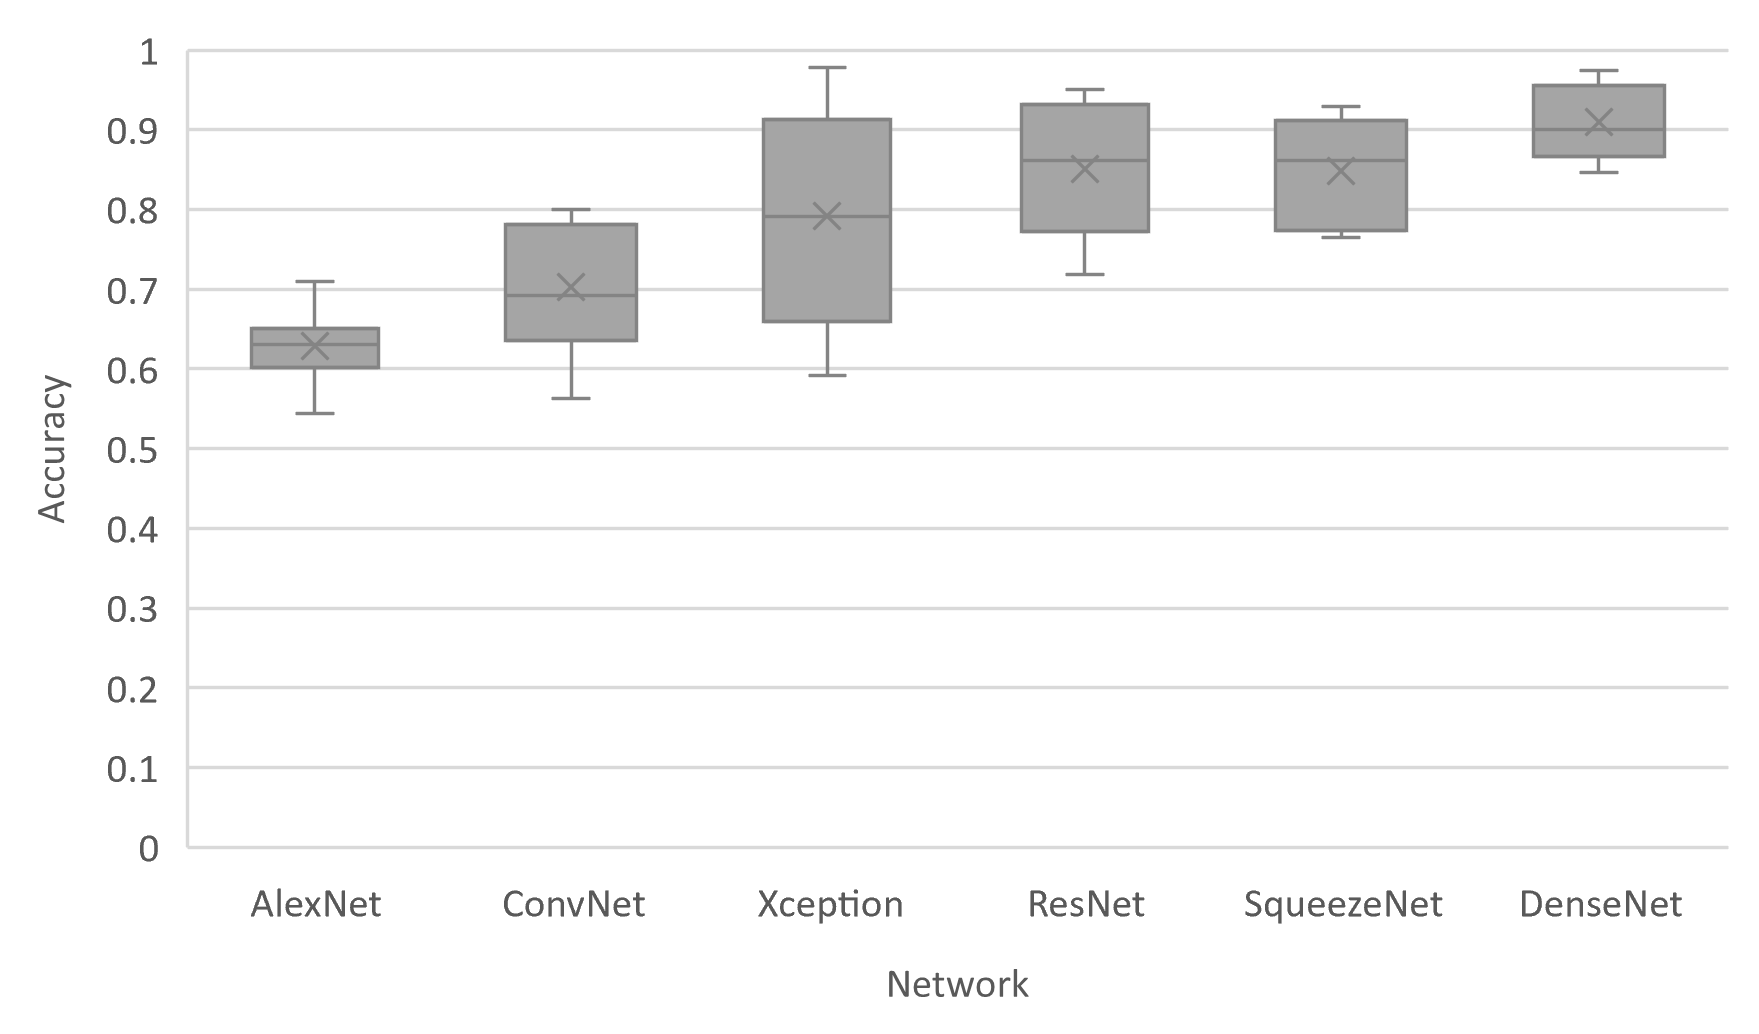
\includegraphics[width=\textwidth]{figures/round-1-model-accuracy.png}
    \caption{Initial training model accuracy, separated by network type.}
    \label{fig:round-1-model-accuracy}
\end{figure}

Another result worth noting from \autoref{fig:round-1-model-accuracy} is the differences between models using transfer learning and those not. Xception, DenseNet and ResNet are the three best performing models, after hyper-parameter tuning, and all three made use of transfer learning with the pre-trained ImageNet weights. However SqueezeNet breaks this trend, as it boasts results close to the three transfer learning models without making use of transfer learning itself. This is likely due to SqueezeNets small size, allowing for faster training to reach a higher accuracy within the maximum allowed epochs.

The improvement of accuracy of Xception versus DenseNet comes at a cost of training time. Comparing training time to accuracy in \autoref{fig:round-1-model-training-time} shows a trend that a longer training time is generally necessary to improve accuracy. There are a number of outliers here however, as smaller models with the best tuned hyper-parameters outperform larger models with worse tuned hyper-parameters.

\begin{figure}[H]
    \centering
    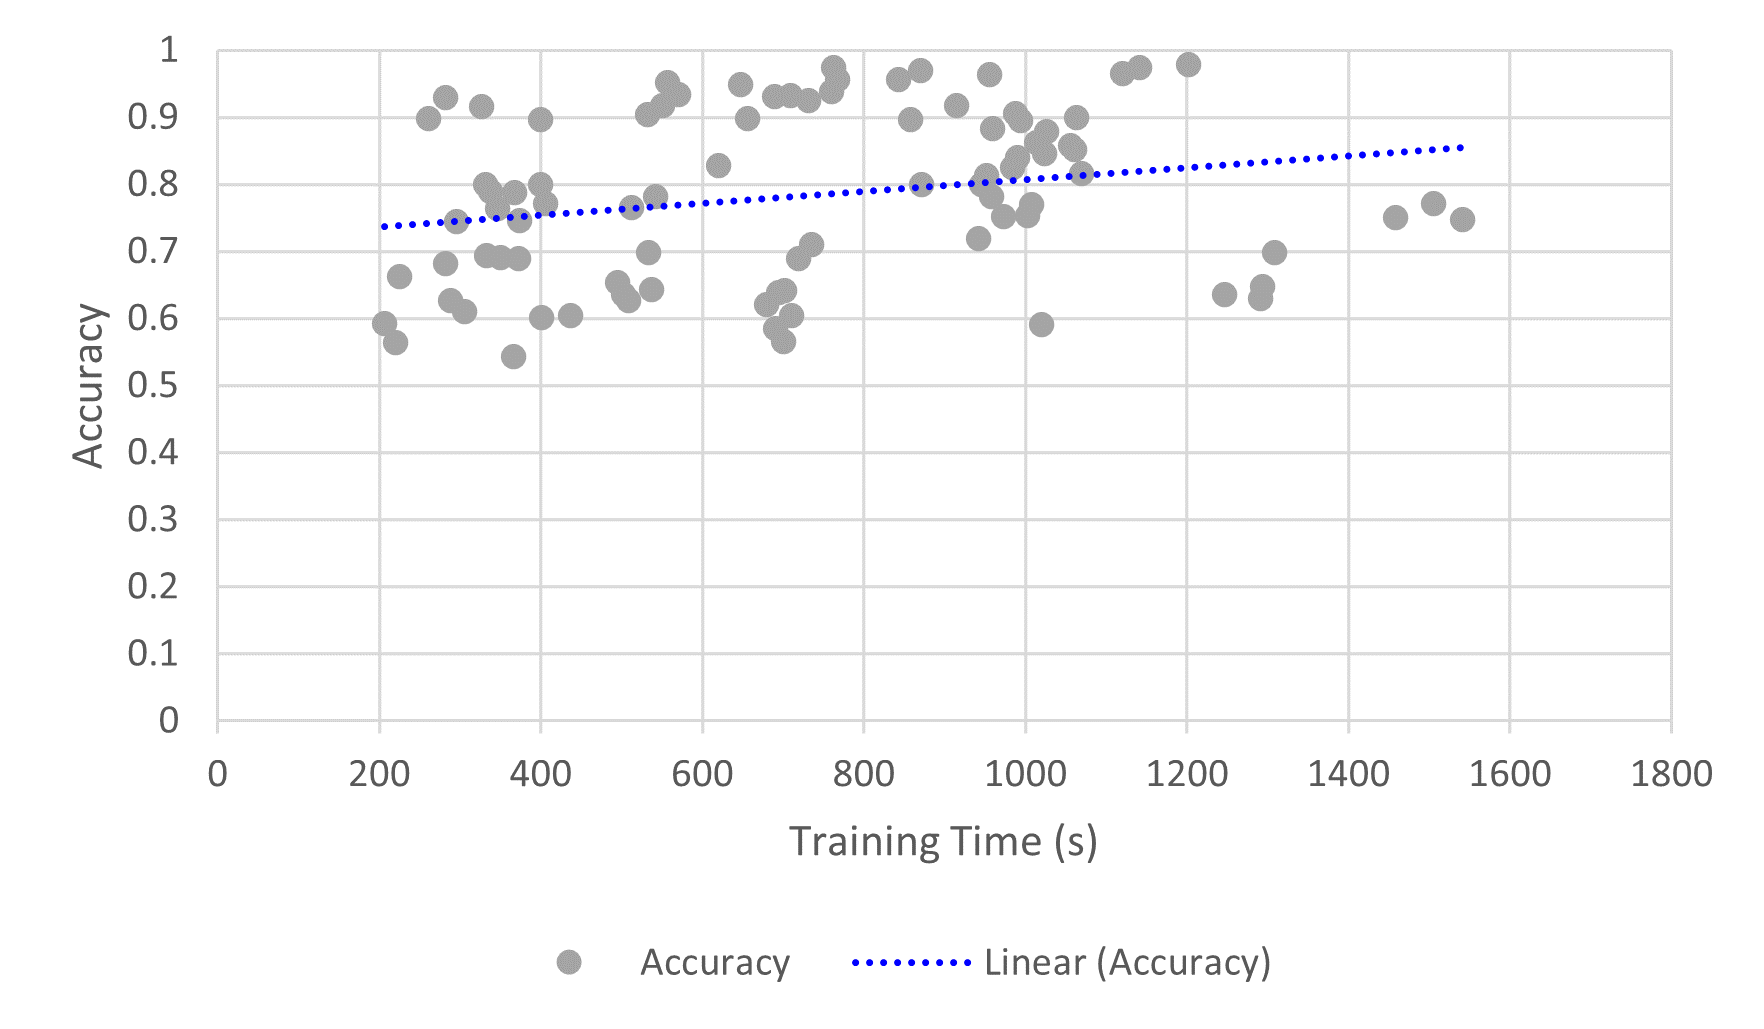
\includegraphics[width=\textwidth]{figures/round-1-model-training-time2.png}
    \caption{Initial training model accuracy versus time.}
    \label{fig:round-1-model-training-time}
\end{figure}

Outliers to this theory could also be due to the age of the networks. One such example in this case is AlexNet, which was published in 2012, versus DenseNet, which was published in 2016. When using the best hyper-parameter combinations for each model, while they both share a similar straining time, DenseNet is $\sim$0.27 more accurate than AlexNet. This can be seen in \autoref{fig:round-1-best-model-training-time}.

\begin{figure}[H]
    \centering
    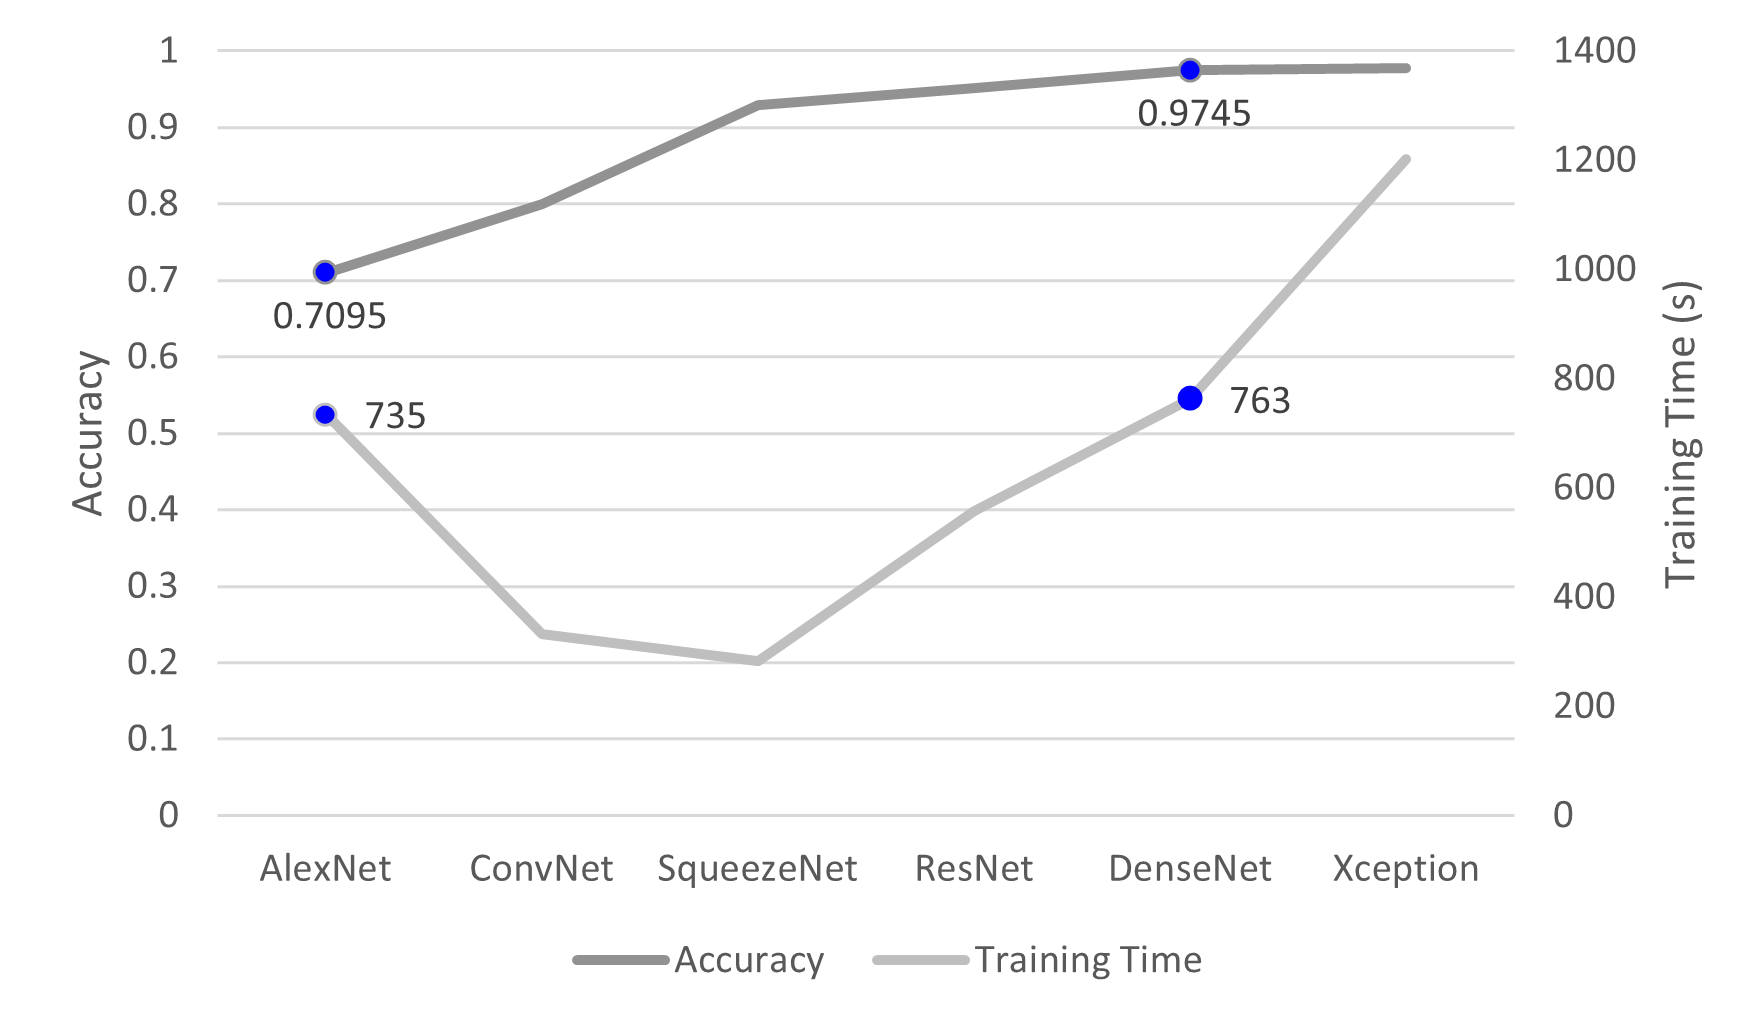
\includegraphics[width=\textwidth]{figures/round-1-best-model-training-time.png}
    \caption{Differences between model age, accuracy and time.}
    \label{fig:round-1-best-model-training-time}
\end{figure}

Hyper-parameters had a large effect on model performance. An example of this is the difference between Xception's best and worse performing hyper-parameters, seen in \autoref{fig:xception-best-worst-hparams}, which have a difference of $\sim$0.38 accuracy.

\begin{figure}[H]
    \centering
    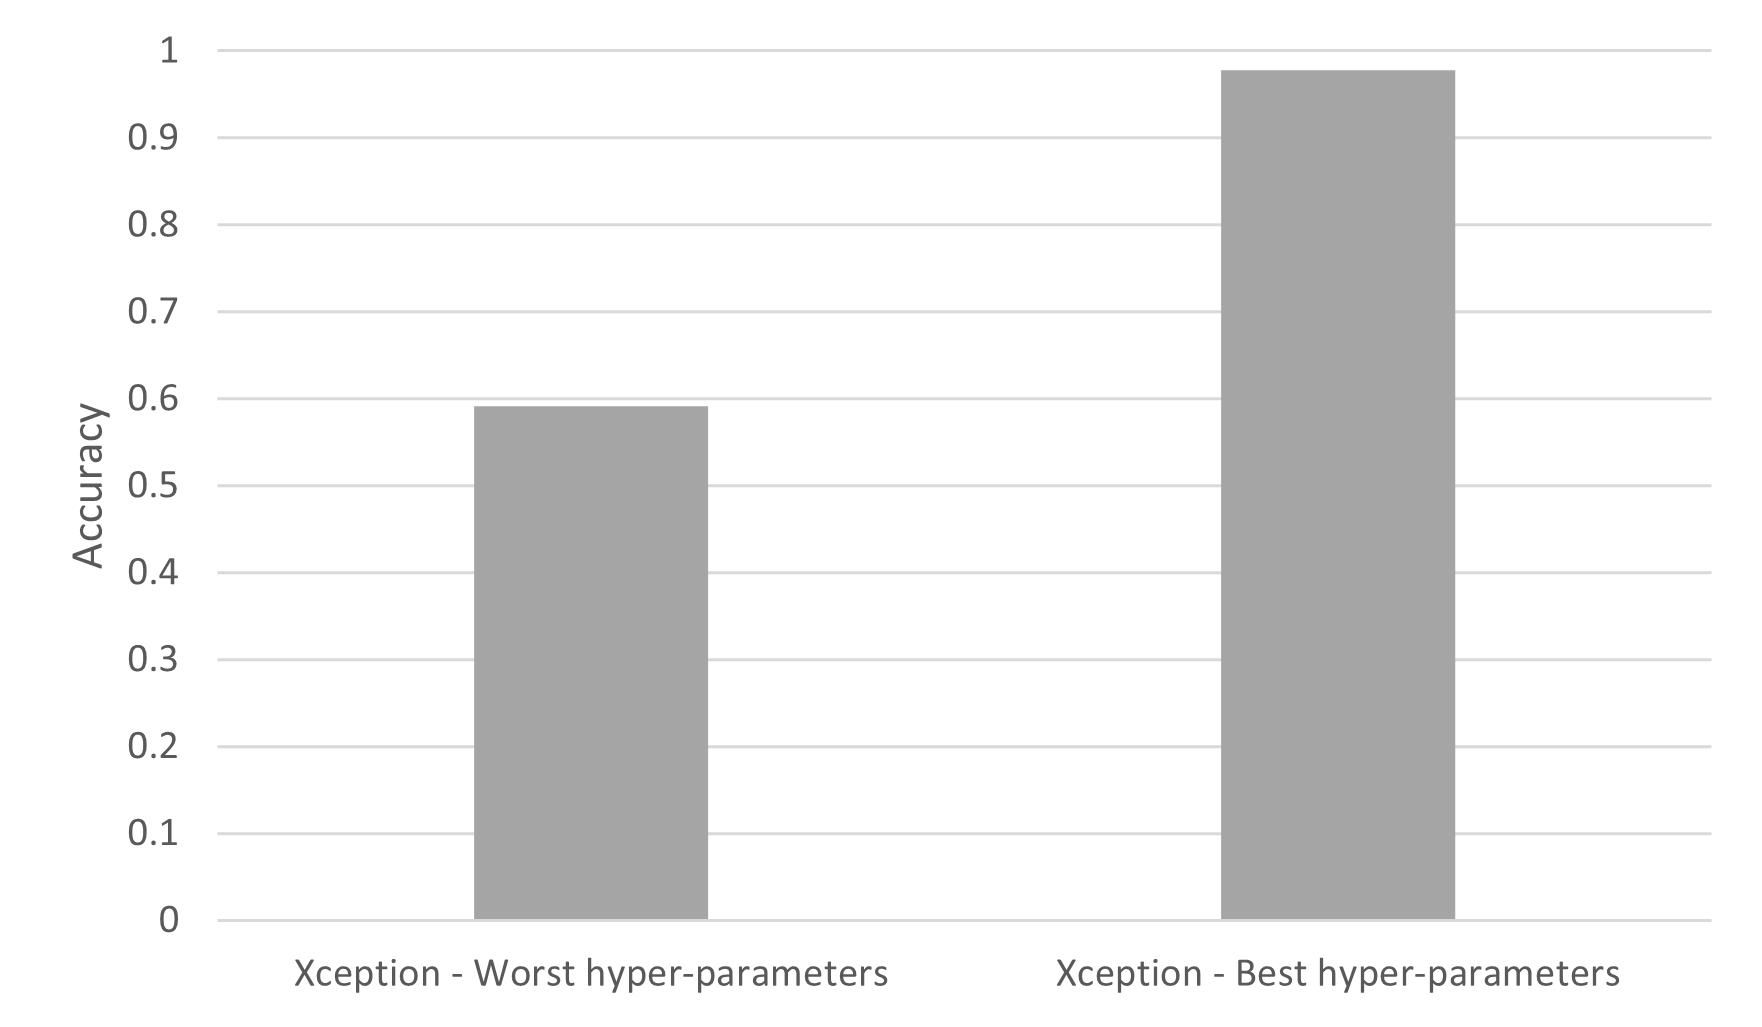
\includegraphics[width=\textwidth]{figures/xception-best-worst-hparams.png}
    \caption{Xception's best and worse performing hyper-parameters.}
    \label{fig:xception-best-worst-hparams}
\end{figure}

The hyper-parameters of one model, which perform well, might not necessarily mean that they would work well for another model however. As seen in \autoref{fig:round-1-dense-units} and \autoref{fig:round-1-learning-rate}, there is little variability in accuracy when using different hyper-parameters, when looking at the accuracy produced by all models.

\begin{figure}[H]
    \centering
    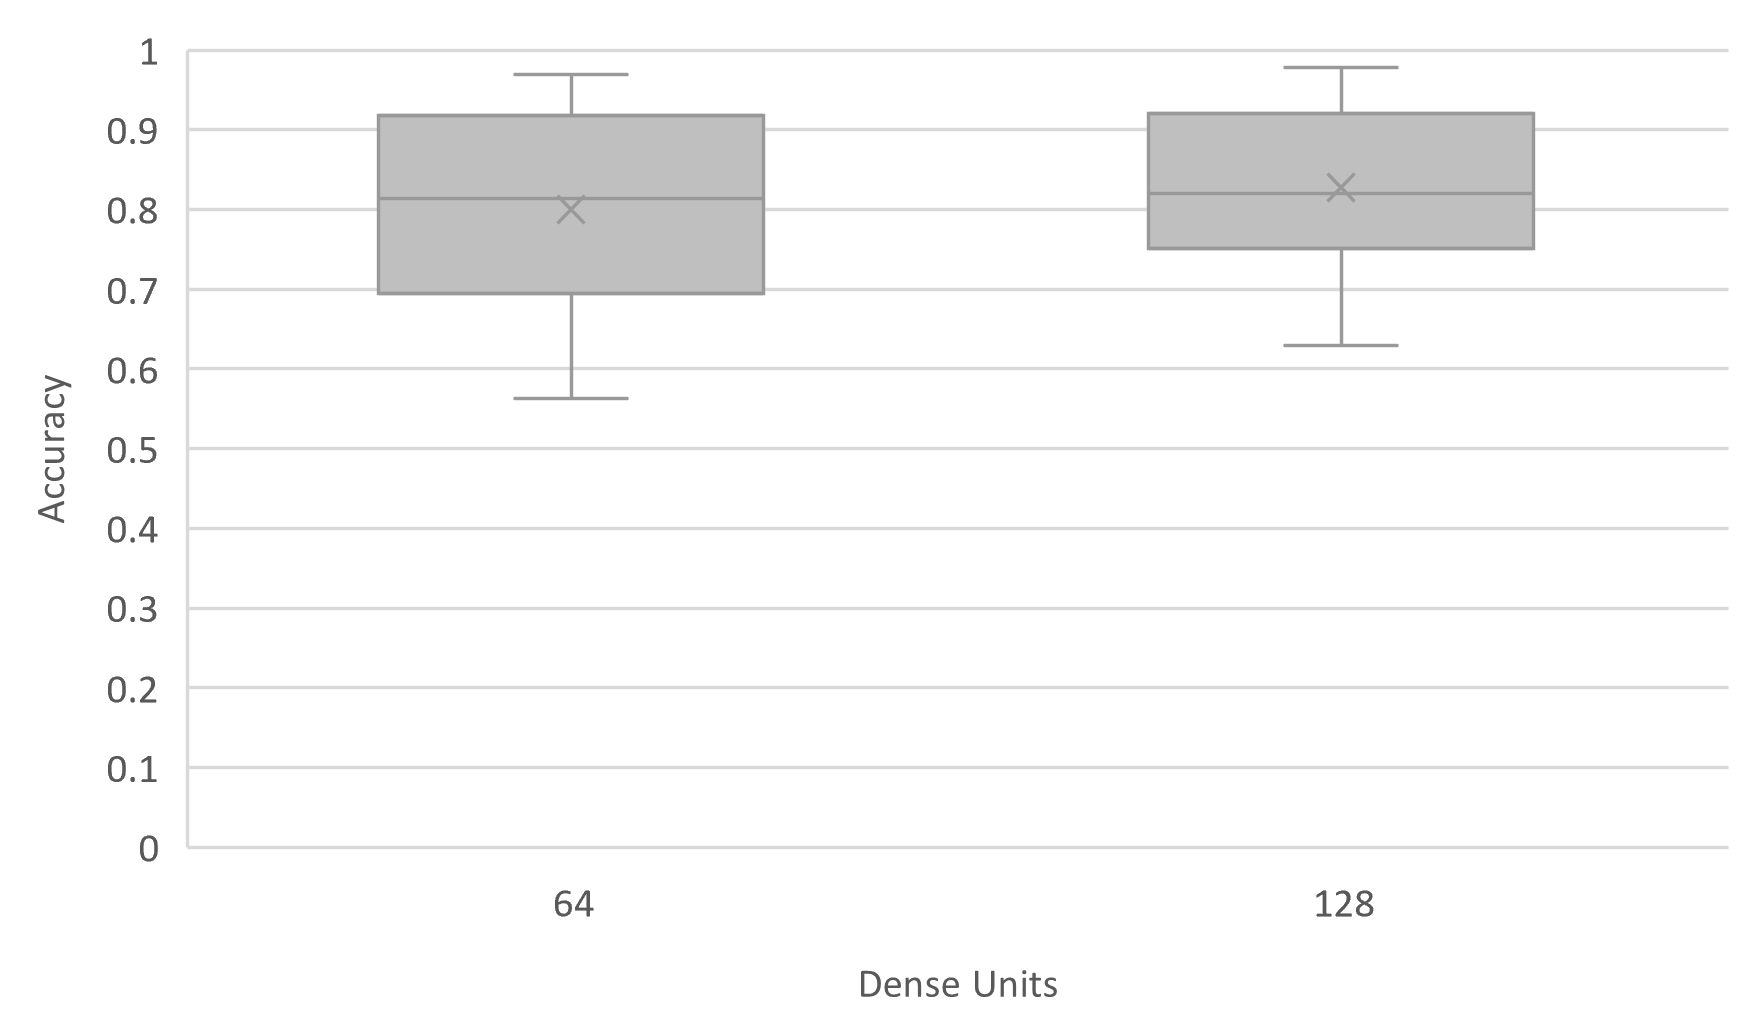
\includegraphics[width=\textwidth]{figures/round-1-dense-units.png}
    \caption{Model performance based on the dense units hyper-parameter.}
    \label{fig:round-1-dense-units}
\end{figure}

\begin{figure}[H]
    \centering
    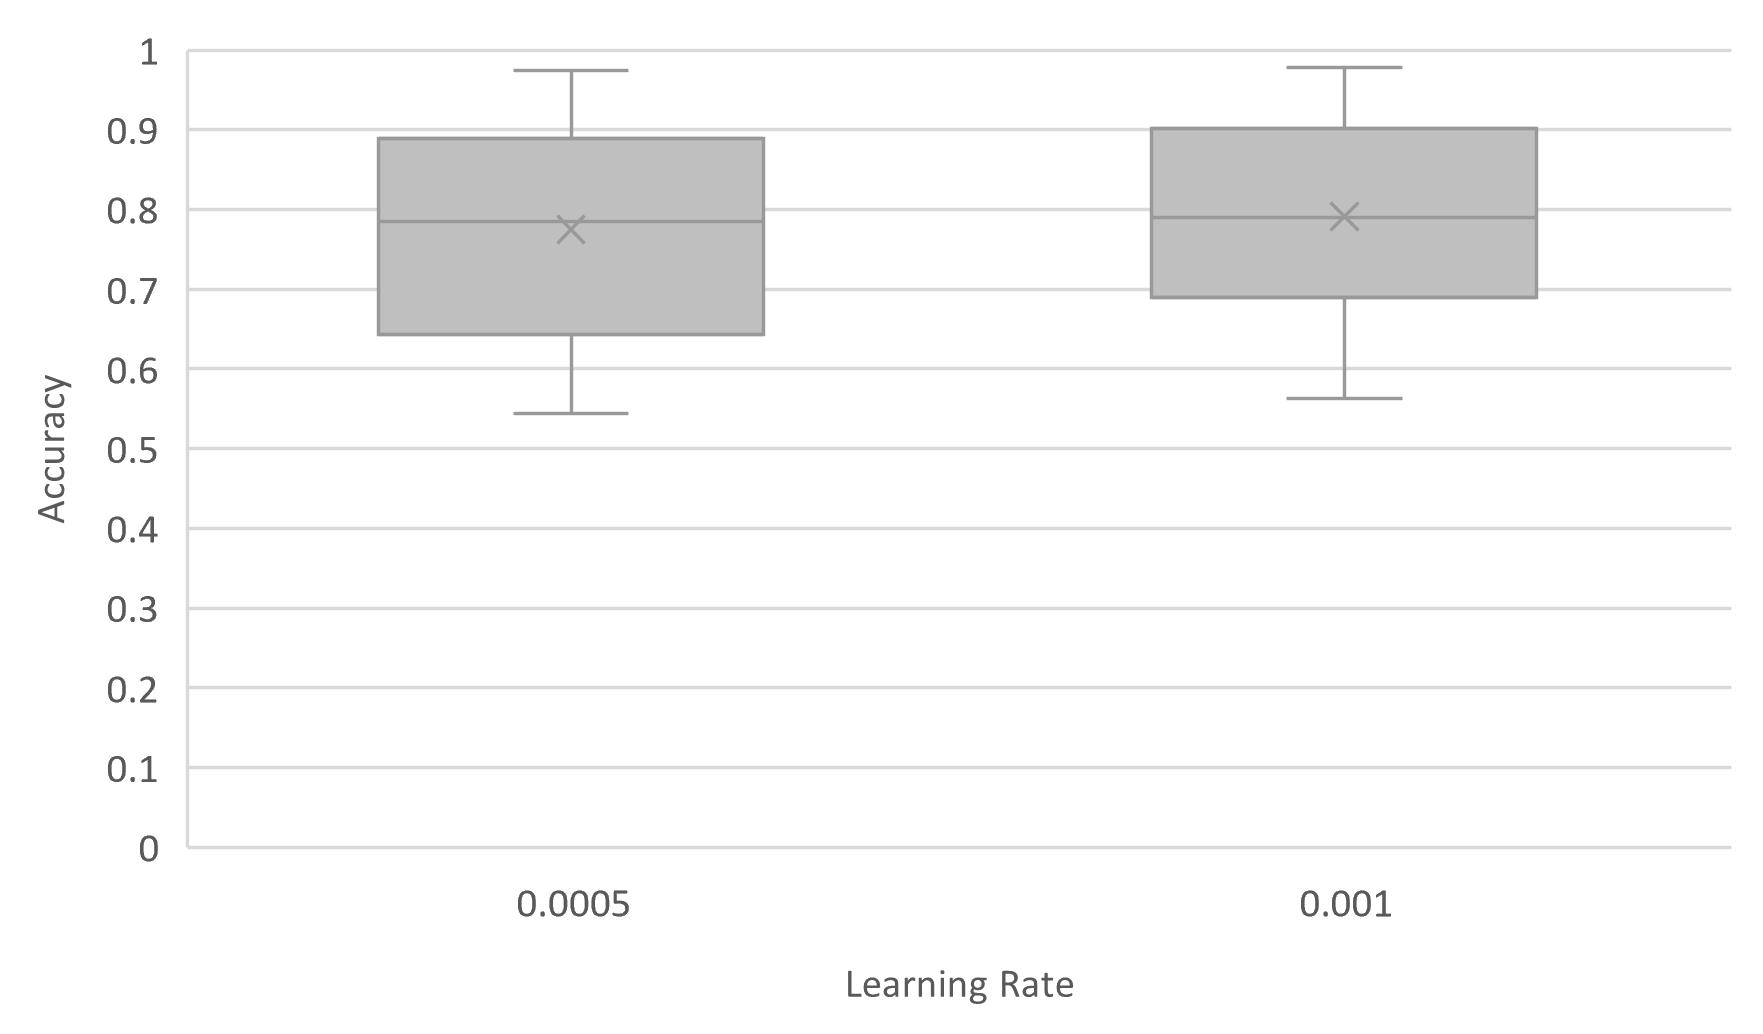
\includegraphics[width=\textwidth]{figures/round-1-learning-rate.png}
    \caption{Model performance based on the learning rate hyper-parameter.}
    \label{fig:round-1-learning-rate}
\end{figure}

Xception was chosen to move to the model improvements round as its best model had the best accuracy, precision, recall and F1 score out of all assessed models. The improvements made to the Xception network past the initial ones made during the initial round did not prove successful. While some advancements were made in reducing training time, this meant a hit in accuracy. One such example is that of Improvement 4, which boasts a 46\% reduction in training time while only having a 16\% decrease in accuracy, seen in \autoref{fig:round-2-accuracy-training}. This change is likely due to the concatenation of the ResNet network alongside the addition layers as proposed by \cite{fitriasari2021improvement}, as the training times seen are similar to those of ResNet. This correlation is not wholly due to the concatenation of ResNet however, as Improvement 3, which also uses this design, does not show the same improvements in training times.

\begin{figure}[H]
    \centering
    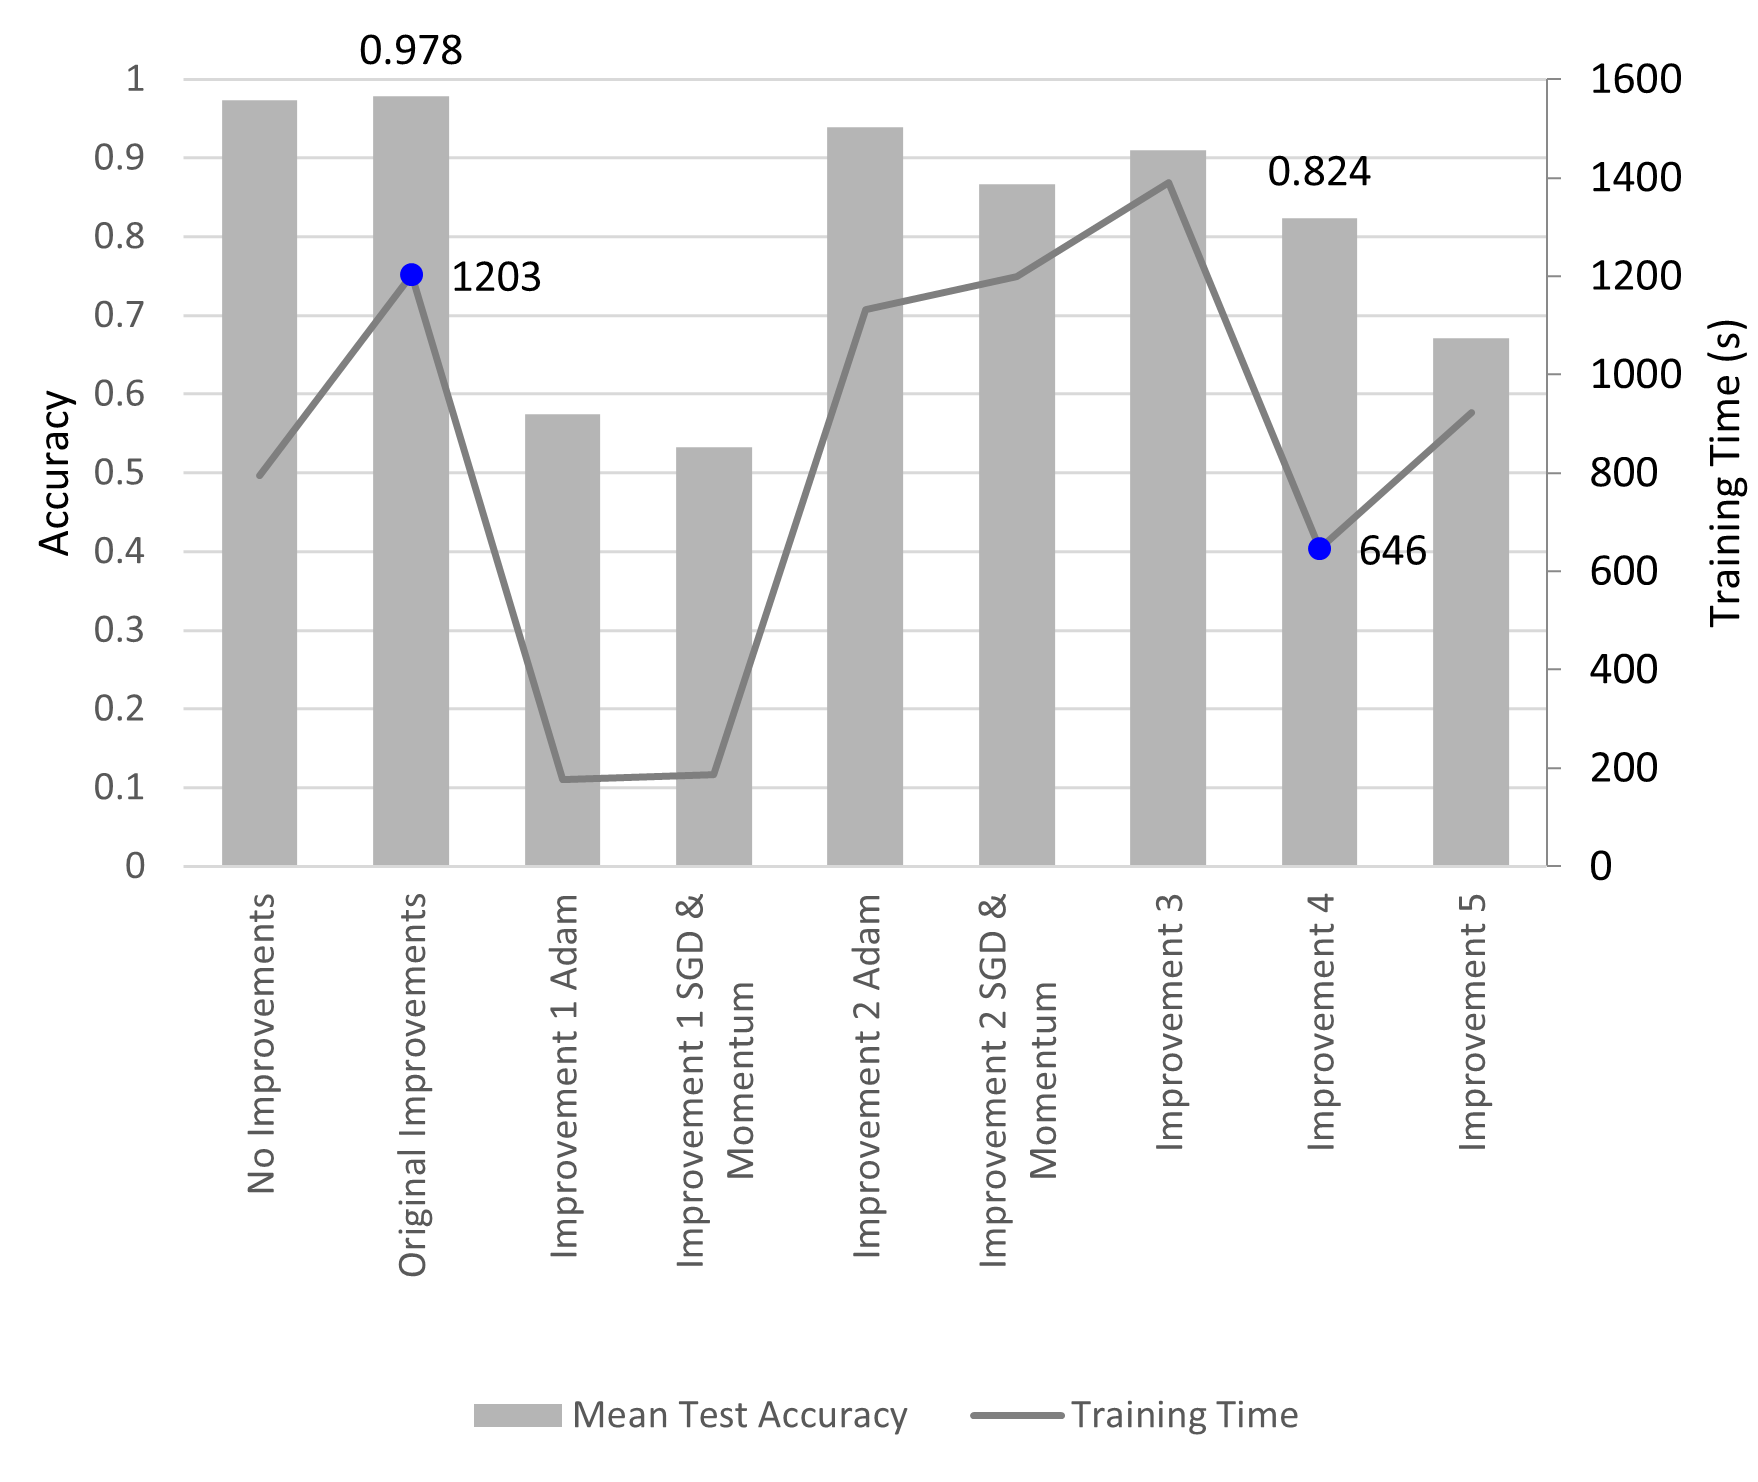
\includegraphics[width=\textwidth]{figures/round-2-accuracy-training.png}
    \caption{Model performance based on the learning rate hyper-parameter.}
    \label{fig:round-2-accuracy-training}
\end{figure}

Talk about results, which model performed the best, why Xception was chosen for improvements, the improvements chosen for final evaluation, the final models, differences between them, maybe say hard to tell which is best?

